\documentclass[../main.tex]{subfiles}
\begin{document}

\subsection{Reeks A}

\subsubsection{Vraag 1}
\begin{question}(...) fervente aanhangers van de oudere rekenhulpmiddelen beweerd dat een aantal rekenvaardigheden verloren zouden gaan, o.a. het schatten van de grootte van het resultaat. Denk je dat de actuele ontwikkelingen op het gebied van ICT ook een aantal vaardigheden doen verloren gaan?
\end{question}

\subsubsection{Vraag 2}
\begin{question}
Welke basissen van getallensystemen zijn er in de loop van de geschiedenis gebruikt en waar vinden we die nu nog terug?
\end{question}

\begin{solution}
	\begin{description}
			\item[Basis 60] vinden we terug in onze indeling van tijd. 1 uur is namelijk 60 minuten, een minuut is 60 seconden. Ook het gebruik van graden in de meetkunde verwijst naar een basis van 60. Babylonische wiskundigen gebruikten in 1750 voor Chr. het sexagesimaal positiestelsel met basis 60. Deze notatie was al floating point. Hierbij kunnen de vingerkootjes gebruikt worden om tot 12 te tellen, terwijl het andere hand kan gebruikt worden om veelvouden bij te houden. Waardoor er ook op de handen geteld kan worden tot 60.
			\item[Basis 20] In het pre-columbiaanse Amarika vinden we getallen notaties terug bij de Maya's die gebruik maken van basis 20. Ook de Franse woorden voor getallenreeksen duiden op een basis 20.
			(quatre-vingt). Bovendien werd tot enkele decennia geleden de Britse pond verdeelt in 20 shilling en elke shilling in 12 pence (basis 12).
			\item[Basis 10] komt ongetwijfeld van het tellen op de 10 vingers van de beide handen. In Babyloni\"e rond 1750 voor Chr. werden er tijdens handelsbetrekkingen getallen genoteerd per groeperingen per 10, per 100 enzovoort. Zij maakten dus eigenlijk gebruik van basis 10. De getallennotatie in het decimale positiestelsel die we nu kennen (voor gehele getallen) is ontstaan in India, rond 600 na Christus.
			\item[basis 12] In vele westerse talen hebben de getallen van 1 tot en met 12 een eigen naam (bv. dozijn). Dit wijst erop dat 12 ook mogelijk ooit als basis werd gebruikt. Bovendien kan voor basis 12 geteld worden op de vingerkootjes, wat ook op de origine van deze basis kan wijzen.
			\item[Basis 2] wordt gebruikt in computers.

	\end{description}	
\end{solution}

\subsubsection{Vraag 3}
\begin{question}
Waarom is nul belangerijk? Ken je de vermoedelijke oorsprong?
\end{question}

\begin{solution}
Rond 1750 voor Chr. gebruikten Babylonische wiskundigen een symbool voor 0 als plaatshouder, maar het werd nog niet als getal gebruikt en ook nooit achteraan of vooraan een getal geschreven. In 1202 publiceerde Leonarda Van Pisa (Fibonacci) ``Liber Abaci'' waarin het gebruik van arabische cijfers werd beschreven, inclusief nul. Hiermee werd het ge\"introduceerd in Europa.
	
\end{solution}

\subsubsection{Vraag 4}
\begin{question}
Welke rekenhulpmiddelen heb je zelf gebruikt? Welke ken je? Welke zijn er in onbruik geraakt en waarom?
\end{question}

\subsubsection{Vraag 5}

\begin{figure}[h!]
	\begin{center}
		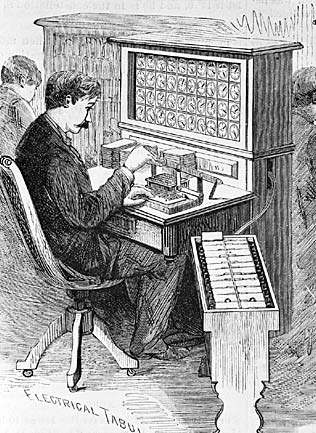
\includegraphics[scale=0.5]{ponskaarthollerith}
		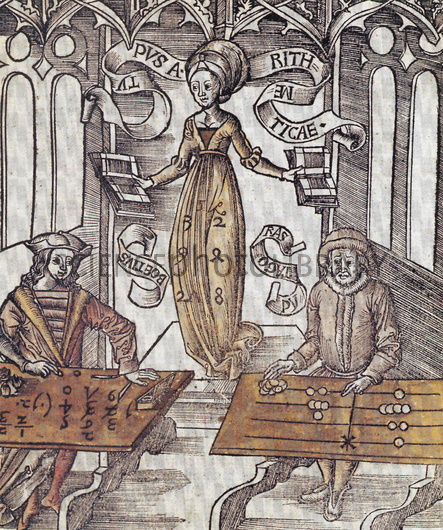
\includegraphics[scale=0.41]{algorithms}
	\end{center}
	\caption{Figuren bij vraag 5}
	\label{fig:vraag5}
\end{figure}

\begin{question}
Kan je de de figuren op figuur \ref{fig:vraag5} thuisbrengen? Vertel wat je ervan weet.
\end{question}


\end{document}